% arara: indent: {overwrite: yes}
\section{Лабораторная 1}

\subsection{Условие}

\textbf{Согласно варианту:} $\mathbf{X_{0} = \alpha = 16 807, K = 64}$.

Используя метод Маклерена-Марсальи построить датчик БСВ (1 датчик должен быть мультипликативно конгруэнтный, второй – на выбор). Исследовать точность построенной БСВ.

\begin{enumerate}
	\item Осуществить моделирование $n = 1000$ реализаций БСВ с помощью мультипликативного конгруэнтного метода (МКМ) с параметрами $X{0}, \alpha, m = 231$;
	\item Осуществить моделирование $n = 1000$ реализаций БСВ с помощью метода Макларена-Марсальи (один датчик должен быть мультипликативно конгруэнтный (п. 1), второй – на выбор).
	      $K$ – объем вспомогательной таблицы;
	\item Проверить точность моделирования обоих датчиков (п. 1 и п. 2) с помощью критерия согласия Колмогорова и $\chi^{2}$ - критерия Пирсона с уровнем значимости $\varepsilon = 0.05$.
\end{enumerate}

\subsection{Теория}
\subsubsection{Датчики БСВ}
Для моделирования на ЭВМ реализаций \textbf{\textit{Базовой случайной величины}} используются специальные программы, называемые программными датчиками БСВ.\\
В основе программных датчиков БСВ лежат рекуррентные формулы вида:

\begin{equation}
	x_{n} = \varphi (x_{n-1}, \ldots, x_{n-p}), n = 1, 2, \ldots ,
	\label{main_recurrent:ref}
\end{equation}

где $x_{1-p}, x_{2-p}, \ldots, x_{0}$ $(p \geqslant 1)$  - заданные стартовые значения. Описанное соотношение (\ref{main_recurrent:ref}) описывает детерминированный алгоритм, однако при соответствующем подборе преобразования $\varphi(\cdot)$ получаемые на его основе псевдослучайные числа ${x_{n}}$ по своим функциональным и числовым характеристикам близки к БСВ.

Алгоритмы моделирования вида (\ref{main_recurrent:ref}) обладают общим недостатком: начиная с некоторого момента $\mathbf{t_{0}}$, последовательность псевдослучайных чисел образует цикл, который повторяется бесконечное число раз. Длина $\mathbf{T}$ циклически повторяющейся последовательности называется \textbf{\textit{периодом датчика}} БСВ $(T \leq m - 1)$.

Период $\mathbf{T}$ и \textbf{\textit{коэффициент использования}} БСВ $\mathbf{k}$ являются основными показателями качества программных датчиков БСВ. Лучшим датчикам соответствуют большие значения $\mathbf{T}$ и $\mathbf{k}$.

\subsubsection {Линейный конгруэнтный метод}\label{linear_congruential_generator}
\textbf{Линейный конгруэнтный метод} - один из методов генерации псевдослучайных чисел. Применяется в простых случаях и не обладает криптографической стойкостью. Входит в библиотеки различных компиляторов.

Суть метода заключается в вычислении последовательности случайных чисел $X_n$ следующим образом:

\begin{equation}
	X_{n+1} = \frac{\alpha X_{n} + c) \bmod m}{m},
	\label{linear_congruential_generator_formula:ref}
\end{equation}

где:

\hfill\parbox{17.5cm}{
	$
		\left.
		\begin{array}{ccc}
			\begin{aligned}
				 & \text{1. } X_{0} \text{ - начальное значение } (0 \leqslant X_{0} < 1) \\
				 & \text{2. } \alpha \text{ - множитель } (0 \leqslant \alpha < m)        \\
				 & \text{3. } c \text{ - приращение } (0 \leqslant c < m )                \\
				 & \text{4. } m \geq 2 \text{ - модуль }                                  \\
			\end{aligned}
		\end{array}
		\right\}
	$ - \textbf{\textit{параметры датчика}}.
}\\\\

\textbf{Типовые значения параметров:} $m = 2^{31}, x_0 = \alpha = 65539$.

\subsubsection{Мультипликативный конгруэнтный метод}
Метод генерации \textit{линейной конгруэнтной последовательности} (раздел \ref{linear_congruential_generator}) при $\mathbf{c = 0}$ называют \textbf{\textit{мультипликативным конгруэнтным методом}}.

\subsubsection{Метод Макларена-Марсальи}
\textbf{\textit{Генератор Макларена-Марсальи}} - криптографически стойкий генератор псевдослучайных чисел, который основан на комбинации двух конгруэнтных генераторов и вспомогательной матрице, с помощью которой происходит перемешивание двух последовательностей, полученных от двух генераторов.

Данный генератор псевдослучайных чисел оперирует с тремя объектами: двумя конгруэнтными генераторами, которые порождают последовательности $\mathbf{\langle X_n \rangle, \langle Y_n \rangle}$, и массива $\mathbf{V}$, состоящей из $\mathbf{k}$ элементов, обычно $k \in \lbrace 64, 28, 256 \rbrace$. На выходе последовательность $\mathbf{\langle Z_n \rangle}$.

Генератор состоит из четырёх основных стадий:
\begin{enumerate}
	\item Инициализация $\mathbf{V}$ и $\mathbf{Z}$ первыми $\mathbf{k}$ элементами последовательности $\mathbf{\langle X_n \rangle}$ - выполняется один раз;
	\item Выборка $\mathbf{X, Y}$ из $\mathbf{\langle X_n \rangle, \langle Y_n \rangle}$, то есть $\mathbf{X, Y}$ - очередные члены последовательностей $\mathbf{\langle X_n \rangle, \langle Y_n \rangle}$;
	\item Вычисление $\mathbf{j = \lfloor k \cdot Y \rfloor}$, где $\mathbf{j \in [0,k)}$ - случайное число, определяемое $Y$;
	\item Присвоение $\mathbf{Z_i=V_i}$ и замена $\mathbf{V_j = X}$.
\end{enumerate}

Последние три стадии могут повторяться необходимое число раз.

Данный метод позволяет ослабить зависимость между членами последовательности $\mathbf{Z_n}$ и получить сколь угодно большие значения её периода $T$ при условии, что периоды $T_1, T_2$ исходных датчиков являются взаимно простыми числами. Коэффициент использования БСВ для данного датчика $\mathbf{k=\frac{1}{2}}$ (за исключением первой реализации, для моделирования которой используется $K+1$ реализация).

\subsubsection{$\chi^2$ критерий согласия Пирсона}
\textbf{\textit{Критерий согласия Пирсона}} - это непараметрический метод, который позволяет оценить значимость различий между фактическим (выявленным в результате исследования) количеством исходов или качественных характеристик выборки, попадающих в каждую категорию, и теоретическим количеством, которое можно ожидать в изучаемых группах при справедливости нулевой гипотезы. Метод позволяет оценить статистическую значимость различий двух или нескольких относительных показателей (частот, долей).

Данный критерий применяют для проверки гипотезы о соответствии эмпирического распределения предполагаемому теоретическому распределению $F(X)$ при большом объёме выборки $(n \geqslant 100)$. \textit{Критерий применим для любых видов функции $F(x)$, даже при неизвестных значениях их параметров, что обычно имеет место при анализе результатов механических испытаний}.\\

Статистика критерия проверки гипотез имеет вид:

\begin{equation}
	\chi^{2} = \sum_{i=1}^{p} \frac{(n_{i} - n \cdot p_{i})^{2}}{n \cdot p_{i}},
\end{equation}

где $n_{i}$ - наблюдаемые частоты, $n \cdot p_{i}$ - ожидаемые частоты.\\

Чем больше $\chi^{2}$, тем сильнее выборка $X$ не согласуется с гипотезой $H_0$ (\textbf{\textit{нулевая гипотеза}}: наблюдаемые частоты соответствуют ожидаемым).

Чтобы проверить гипотезу по \textit{критерию Пирсона} необходимо сравнить \textit{статистику критерия} с \textit{критическим значения}, которой находится в таблице для соответствующего \textit{уровня значимости} и количеству \textit{степеней свободы}.\\

\textbf{Пример:}
при уровне значимости $\alpha = 0.05$ и количестве степеней свободы $\nu = 9$ \textit{критерий Пирсона} согласуется с \textit{нулевой гипотезой} при $\chi^{2} < 16.919$.

\begin{figure}[h!]
	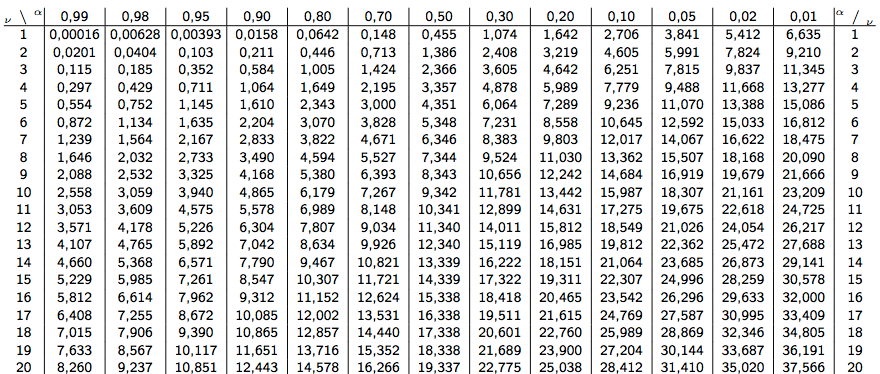
\includegraphics [width=\textwidth] {pirson_critical_values.png}
	\caption{Значения $\chi^2$ при различных $P_{\chi^{2}}$ в зависимости от числа степеней свобод $\nu$.}
	\label{fig:pirson_critical_values}
\end{figure}

\subsubsection{Критерий согласия Колмогорова}
\textbf{\textit{Критерий согласия Колмогорова}} предназначен для проверки гипотезы о принадлежности выборки некоторому закону распределения, то есть проверки того, что эмпирическое распределение соответствует предполагаемой модели.

\textbf{\textit{Эмпирическая функция распределения}} $\mathbf{F_{n}}$, построенная по выборке $X = (X_{1}, \ldots, X_{n})$, имеет вид:
\begin{equation}
	F_{n}(x) = \frac{1}{n} \sum_{i=1}^{n}I_{X_{i} \leqslant x}
\end{equation}

где $I_{X_{i} \leqslant x}$ указывает, попало ли наблюдение $X_{i}$ в область $(-\infty, x]$:
\begin{equation}
	I_{X_{i} \leqslant x} =
	\begin{cases}{}
		1, X_{i} \leqslant x \\
		0, X_{i} > x         \\
	\end{cases}
\end{equation}

\textbf{\textit{Статистика критерия}} для эмпирической функции распределения $F_{n}(x)$ определяется следующим образом:
\begin{equation}
	D_{n} = \sup_{x \in R} |F_{n}(x) - F(x)|
\end{equation}

\textbf{Принятие решения по критерию Колмогорова:}
В случае справедливости \textit{нулевой гипотезы} ($H_{0}$) при $n \rightarrow + \infty$ статистика $D_{n}$ имеет распределение Колмогорова:
\begin{equation}
	\lim_{n \rightarrow \infty} P(\sqrt{n} D_{n} < x) = K(x)
\end{equation}
здесь
\begin{equation}
	K(x) = \sum_{k = -\infty}^{+\infty} (-1)^{k} e^{-2k^{2}x^{2}} \approx 1 - 2e^{-2x^{2}}, x \geqslant 0
	\label{kolmogorov_distribution_function}
\end{equation}
- функция Колмогорова.\\

При \textbf{\textit{уровне значимости}} $\alpha$ пороговое значение $C_{\alpha}$, находится из соотношения:
\begin{equation}
	K(C_{\alpha}) = 1 - \alpha
	\label{threshold_value}
\end{equation}

Таким образом, для проверки гипотезы о виде распределения получаем:

\begin{equation}
	\rho (X) =
	\begin{cases}{}
		H_{0}, если \sqrt{n} D_{n} \leqslant \alpha, \\
		H_{1}, если \sqrt{n} D_{n} > \alpha.         \\
	\end{cases}
\end{equation}

\begin{figure}[t!]
	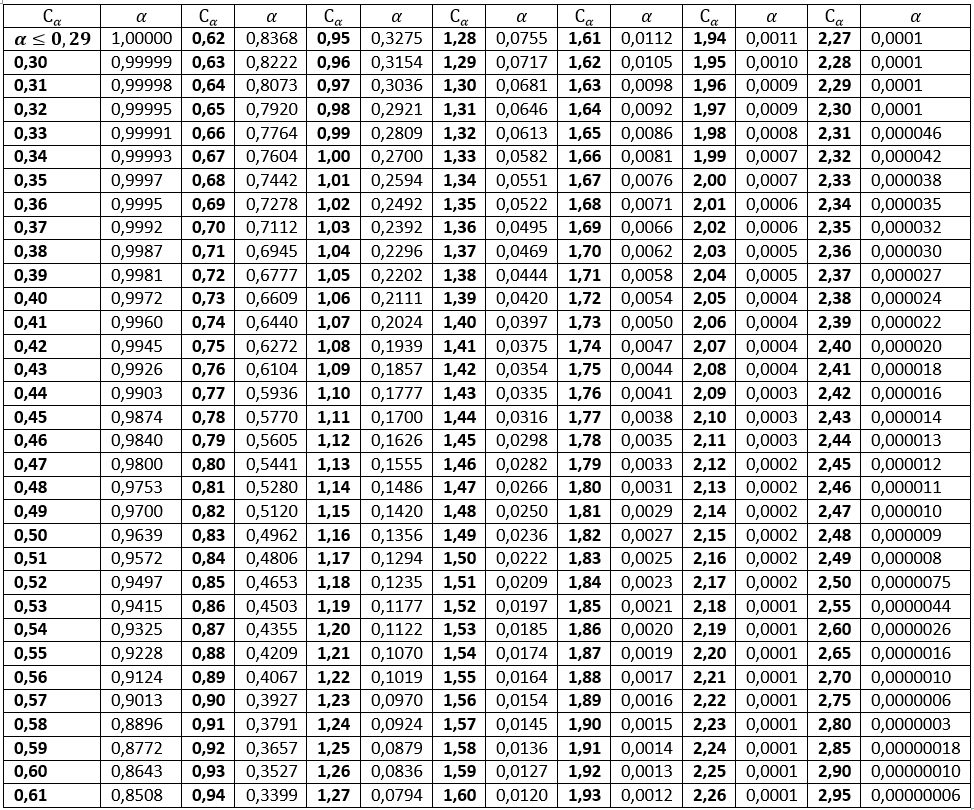
\includegraphics [width=\textwidth] {kolmogorov_critical_values.png}
	\caption{Значения $C_{\alpha}$ при различных $\alpha$.}
	\label{fig:pirson_critical_values}
\end{figure}

\newpage
\textbf{Пример:}
при уровне значимости $\alpha = 0.05$ и пороговое значение из соотношений (\ref{kolmogorov_distribution_function}), (\ref{threshold_value}) $\mathbf{C_{\alpha} \approx 1.359}$.\\

\textbf{Критерий согласия Колмогорова для непрерывного равномерное распределения}\\

\textbf{\textit{Непрерывное равномерное распределение}} - распределение случайной вещественной величины, принимающей значения, принадлежащие некоторому промежутку конечно длины, характеризующая тем, что плотность вероятности на этом промежутке почти всюду постоянна.

\textbf{\textit{Функция распределения:}}
\begin{equation}
	F_{X}(x)\equiv P(X \leqslant x) =
	\begin{cases}{}
		0, x < a                           \\
		\frac{x-a}{b-a}, a \leqslant x < b \\
		1, x \geqslant b                   \\
	\end{cases}
\end{equation}

\textbf{\textit{Значения теоретическая функция распределения}} для интервала $[0, 1)$:
\begin{equation}
	F(x) = \frac{x - 0}{1 - 0} = x
\end{equation}

\textbf{\textit{Значения эмпирической функции распределения}}.

Для $x_{i}$ из выборки $X$, значение эмпирической функции распределения:
\begin{equation}
	F_{n}(x) = \frac{n_{i}}{n}
\end{equation}

где $n$ - количество элементов в выборке, $n_{i}$ - количество элементов в выборке меньших $x_{i}$.

\subsection{Код программы}

\lstinputlisting[language=Python]{./lab_1/lab1.py}

\subsection{Результат выполнения}

\begin{figure}[h!]
	\centering
	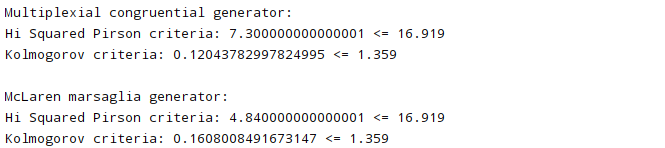
\includegraphics [width=\textwidth] {results.png}
	\label{fig:results}
	\caption{Результат выполнения программы: проверка критерием согласия Пирсона и критерием согласия Колмогорова.}
\end{figure}

\begin{figure}[!h]
  \centering
  \begin{subfigure}[b]{0.45\textwidth}
    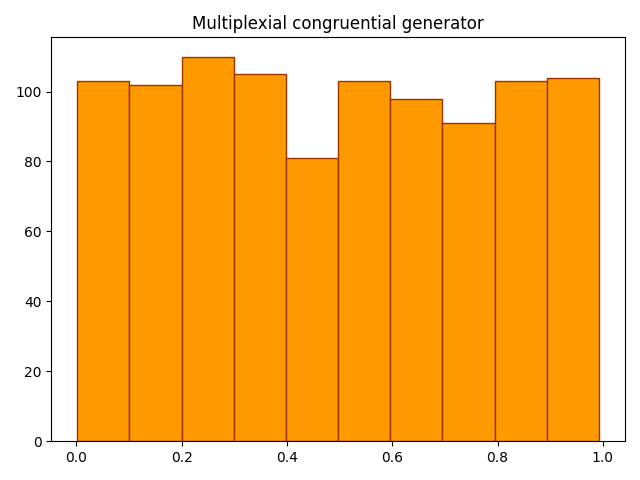
\includegraphics[width=\textwidth]{multiplexial_congruential_generator.png}
    \caption{Диаграмма выборки, полученной мультипликативным конгруэнтным методом.}
  \end{subfigure}
  \hfill
  \begin{subfigure}[b]{0.45\textwidth}
    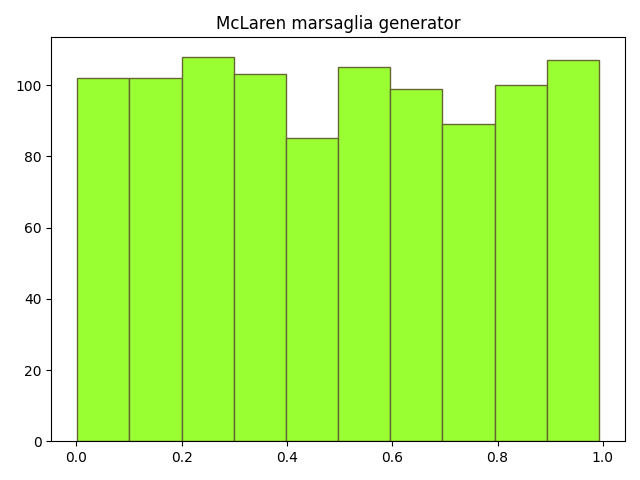
\includegraphics[width=\textwidth]{mclaren_marsaglia_generator.png}
    \caption{Диаграмма выборки, полученной методом Макларена-Марсальи.}
  \end{subfigure}
\end{figure}
